
\documentclass[letterpaper,hide notes,xcolor={table,svgnames},pdftex,10pt]{beamer}
\def\showexamples{t}

\usecolortheme{crane}
\setbeamertemplate{navigation symbols}{}

\usetheme{MyPittsburgh}
\usepackage{hyperref}
\usepackage{graphicx,xspace}
\usepackage[normalem]{ulem}
\usepackage{multicol}
\usepackage{amsmath,amssymb,amsthm,graphicx,xspace}
\newcommand\SF[1]{$\bigstar$\footnote{SF: #1}}

\usepackage[sfdefault,lf]{carlito}
\usepackage[T1]{fontenc}
\usepackage[scaled]{beramono}
\usepackage{tikzpagenodes}
\newcommand{\Rplus}{\protect\hspace{-.1em}\protect\raisebox{.35ex}{\small{\small\textbf{+}}}}
\newcommand{\Cpp}{\mbox{C\Rplus\Rplus}\xspace}

\newcounter{tmpnumSlide}
\newcounter{tmpnumNote}

\newcommand\mnote[1]{%
	\addtocounter{tmpnumSlide}{1}
	\ifdefined\showcues {~\tiny\fbox{\arabic{tmpnumSlide}}}\fi
	\note{\setlength{\parskip}{1ex}\addtocounter{tmpnumNote}{1}\textbf{\Large \arabic{tmpnumNote}:} {#1\par}}}

\newcommand\mmnote[1]{\note{\setlength{\parskip}{1ex}#1\par}}


\newcommand\mquestion[2]{{~\color{red}\fbox{?}}\note{\setlength{\parskip}{1ex}\par{\Large \textbf{?}} #1} \note{\setlength{\parskip}{1ex}\par{\Large \textbf{A}} #2\par}\ifdefined \presentationonly \pause \fi}

\newcommand\blackboard[1]{%
	\ifdefined   \showblackboard
		{#1}
	\else {\begin{center} \fbox{\colorbox{blue!30}{%
						\begin{minipage}{.95\linewidth}%
							\hspace{\stretch{1}} Some space intentionally left blank; done at the blackboard.%
						\end{minipage}}}\end{center}}%
	\fi%
}

\usepackage{listings}
\lstset{%
	keywordstyle=\bfseries,
	aboveskip=15pt,
	belowskip=15pt,
	captionpos=b,
	identifierstyle=\ttfamily,
	frame=lines,
	numbers=left, basicstyle=\scriptsize, numberstyle=\tiny, stepnumber=0, numbersep=2pt}

\usepackage{siunitx}
\newcommand\sius[1]{\num[group-separator = {,}]{#1}\si{\micro\second}}
\newcommand\sims[1]{\num[group-separator = {,}]{#1}\si{\milli\second}}
\newcommand\sins[1]{\num[group-separator = {,}]{#1}\si{\nano\second}}
\sisetup{group-separator = {,}, group-digits = true}

%% -------------------- tikz --------------------
\usepackage{tikz}
\usetikzlibrary{positioning}
\usetikzlibrary{arrows,backgrounds,automata,decorations.shapes,decorations.pathmorphing,decorations.markings,decorations.text}

\tikzstyle{place}=[circle,draw=blue!50,fill=blue!20,thick, inner sep=0pt,minimum size=6mm]
\tikzstyle{transition}=[rectangle,draw=black!50,fill=black!20,thick, inner sep=0pt,minimum size=4mm]

\tikzstyle{block}=[rectangle,draw=black, thick, inner sep=5pt]
\tikzstyle{bullet}=[circle,draw=black, fill=black, thin, inner sep=2pt]

\tikzstyle{pre}=[<-,shorten <=1pt,>=stealth',semithick]
\tikzstyle{post}=[->,shorten >=1pt,>=stealth',semithick]
\tikzstyle{bi}=[<->,shorten >=1pt,shorten <=1pt, >=stealth',semithick]

\tikzstyle{mut}=[-,>=stealth',semithick]

\tikzstyle{treereset}=[dashed,->, shorten >=1pt,>=stealth',thin]

\usepackage{ifmtarg}
\usepackage{xifthen}
\makeatletter
% new counter to now which frame it is within the sequence
\newcounter{multiframecounter}
% initialize buffer for previously used frame title
\gdef\lastframetitle{\textit{undefined}}
% new environment for a multi-frame
\newenvironment{multiframe}[1][]{%
	\ifthenelse{\isempty{#1}}{%
		% if no frame title was set via optional parameter,
		% only increase sequence counter by 1
		\addtocounter{multiframecounter}{1}%
	}{%
		% new frame title has been provided, thus
		% reset sequence counter to 1 and buffer frame title for later use
		\setcounter{multiframecounter}{1}%
		\gdef\lastframetitle{#1}%
	}%
	% start conventional frame environment and
	% automatically set frame title followed by sequence counter
	\begin{frame}%
		\frametitle{\lastframetitle~{\normalfont(\arabic{multiframecounter})}}%
		}{%
	\end{frame}%
}
\makeatother

\makeatletter
\newdimen\tu@tmpa%
\newdimen\ydiffl%
\newdimen\xdiffl%
\newcommand\ydiff[2]{%
	\coordinate (tmpnamea) at (#1);%
	\coordinate (tmpnameb) at (#2);%
	\pgfextracty{\tu@tmpa}{\pgfpointanchor{tmpnamea}{center}}%
	\pgfextracty{\ydiffl}{\pgfpointanchor{tmpnameb}{center}}%
	\advance\ydiffl by -\tu@tmpa%
}
\newcommand\xdiff[2]{%
	\coordinate (tmpnamea) at (#1);%
	\coordinate (tmpnameb) at (#2);%
	\pgfextractx{\tu@tmpa}{\pgfpointanchor{tmpnamea}{center}}%
	\pgfextractx{\xdiffl}{\pgfpointanchor{tmpnameb}{center}}%
	\advance\xdiffl by -\tu@tmpa%
}
\makeatother
\newcommand{\copyrightbox}[3][r]{%
	\begin{tikzpicture}%
		\node[inner sep=0pt,minimum size=2em](ciimage){#2};
		\usefont{OT1}{phv}{n}{n}\fontsize{4}{4}\selectfont
		\ydiff{ciimage.south}{ciimage.north}
		\xdiff{ciimage.west}{ciimage.east}
		\ifthenelse{\equal{#1}{r}}{%
			\node[inner sep=0pt,right=1ex of ciimage.south east,anchor=north west,rotate=90]%
			{\raggedleft\color{black!50}\parbox{\the\ydiffl}{\raggedright{}#3}};%
		}{%
			\ifthenelse{\equal{#1}{l}}{%
				\node[inner sep=0pt,right=1ex of ciimage.south west,anchor=south west,rotate=90]%
				{\raggedleft\color{black!50}\parbox{\the\ydiffl}{\raggedright{}#3}};%
			}{%
				\node[inner sep=0pt,below=1ex of ciimage.south west,anchor=north west]%
				{\raggedleft\color{black!50}\parbox{\the\xdiffl}{\raggedright{}#3}};%
			}
		}
	\end{tikzpicture}
}


%% --------------------

%\usepackage[excludeor]{everyhook}
%\PushPreHook{par}{\setbox0=\lastbox\llap{MUH}}\box0}

%\vspace*{\stretch{1}

%\setbox0=\lastbox \llap{\textbullet\enskip}\box0}

\setlength{\parskip}{\fill}

\newcommand\noskips{\setlength{\parskip}{1ex}}
\newcommand\doskips{\setlength{\parskip}{\fill}}

\newcommand\xx{\par\vspace*{\stretch{1}}\par}
\newcommand\xxs{\par\vspace*{2ex}\par}
\newcommand\tuple[1]{\langle #1 \rangle}
\newcommand\code[1]{{\sf \footnotesize #1}}
\newcommand\ex[1]{\uline{Example:} \ifdefined \presentationonly \pause \fi
	\ifdefined\showexamples#1\xspace\else{\uline{\hspace*{2cm}}}\fi}

\newcommand\ceil[1]{\lceil #1 \rceil}


\AtBeginSection[]
{
	\begin{frame}
		\frametitle{Outline}
		\tableofcontents[currentsection]
	\end{frame}
}



\pgfdeclarelayer{edgelayer}
\pgfdeclarelayer{nodelayer}
\pgfsetlayers{edgelayer,nodelayer,main}

\tikzstyle{none}=[inner sep=0pt]
\tikzstyle{rn}=[circle,fill=Red,draw=Black,line width=0.8 pt]
\tikzstyle{gn}=[circle,fill=Lime,draw=Black,line width=0.8 pt]
\tikzstyle{yn}=[circle,fill=Yellow,draw=Black,line width=0.8 pt]
\tikzstyle{empty}=[circle,fill=White,draw=Black]
\tikzstyle{bw} = [rectangle, draw, fill=blue!20,
text width=4em, text centered, rounded corners, minimum height=2em]

\newcommand{\CcNote}[1]{% longname
	This work is licensed under the \textit{Creative Commons #1 3.0 License}.%
}
\newcommand{\CcImageBy}[1]{%
	\includegraphics[scale=#1]{creative_commons/cc_by_30.pdf}%
}
\newcommand{\CcImageSa}[1]{%
	\includegraphics[scale=#1]{creative_commons/cc_sa_30.pdf}%
}
\newcommand{\CcImageNc}[1]{%
	\includegraphics[scale=#1]{creative_commons/cc_nc_30.pdf}%
}
\newcommand{\CcGroupBySa}[2]{% zoom, gap
	\CcImageBy{#1}\hspace*{#2}\CcImageNc{#1}\hspace*{#2}\CcImageSa{#1}%
}
\newcommand{\CcLongnameByNcSa}{Attribution-NonCommercial-ShareAlike}

\newenvironment{changemargin}[1]{% 
	\begin{list}{}{% 
		\setlength{\topsep}{0pt}% 
		\setlength{\leftmargin}{#1}% 
		\setlength{\rightmargin}{1em}
		\setlength{\listparindent}{\parindent}% 
		\setlength{\itemindent}{\parindent}% 
		      \setlength{\parsep}{\parskip}% 
		      }% 
		\item[]}{\end{list}}




\title{Lecture 4 --- Interrupts \& System Calls }

\author{Jeff Zarnett \& Mike Cooper-Stachowsky \\ \small \texttt{jzarnett@uwaterloo.ca, mstachowsky@uwaterloo.ca}}
\institute{Department of Electrical and Computer Engineering \\
  University of Waterloo}
\date{\today}


\begin{document}

\begin{frame}
	\titlepage

\end{frame}


\begin{frame}
	\frametitle{OBJECTION!!!}

	\begin{center}
		
\includegraphics[width=0.7\textwidth]{images/phoenix-wright-objection.jpg}
	\end{center}


\end{frame}


\begin{frame}
	\frametitle{Interrupts}
	The CPU needs data, but it takes a variable amount of time to get it.\\
	\quad Sometimes this means the equivalent of walking a book from Ottawa.

	In the meantime, I should do something else.

	Polling: check periodically if the book has arrived.

	Interrupts: get a notification when the book is here.

	If someone knocks on my door, I pause what I'm doing and get the book.


\end{frame}

\begin{frame}
	\frametitle{Sources of Interrupts}

	We can put interrupts into four categories, based on their origin:

	\begin{enumerate}
		\item \textbf{Program.}
		\item \textbf{Timer.}
		\item \textbf{Input/Output.}
		\item \textbf{Hardware Failure.}
	\end{enumerate}


\end{frame}

\begin{frame}
	\frametitle{Interrupts}
	Interrupts are a way to improve processor utilization.

	CPU time is valuable!

	When an interrupt take place, the CPU might ignore it (rarely).

	More commonly: we need to \alert{handle} it in some way.

	Analogy: professor in a lecture; student has a question.


\end{frame}

\begin{frame}
	\frametitle{Interrupts}
	The OS: stores the state, handles the interrupt, and restores the state.

	Sometimes the CPU is in the middle of something uninterruptible.\\
	\quad Interrupts may be disabled (temporarily).

	Interrupts can have different priorities.
\end{frame}

\begin{frame}
	\frametitle{Interrupts}

	We may also have multiple interrupts in a short period of time:

	\begin{center}
		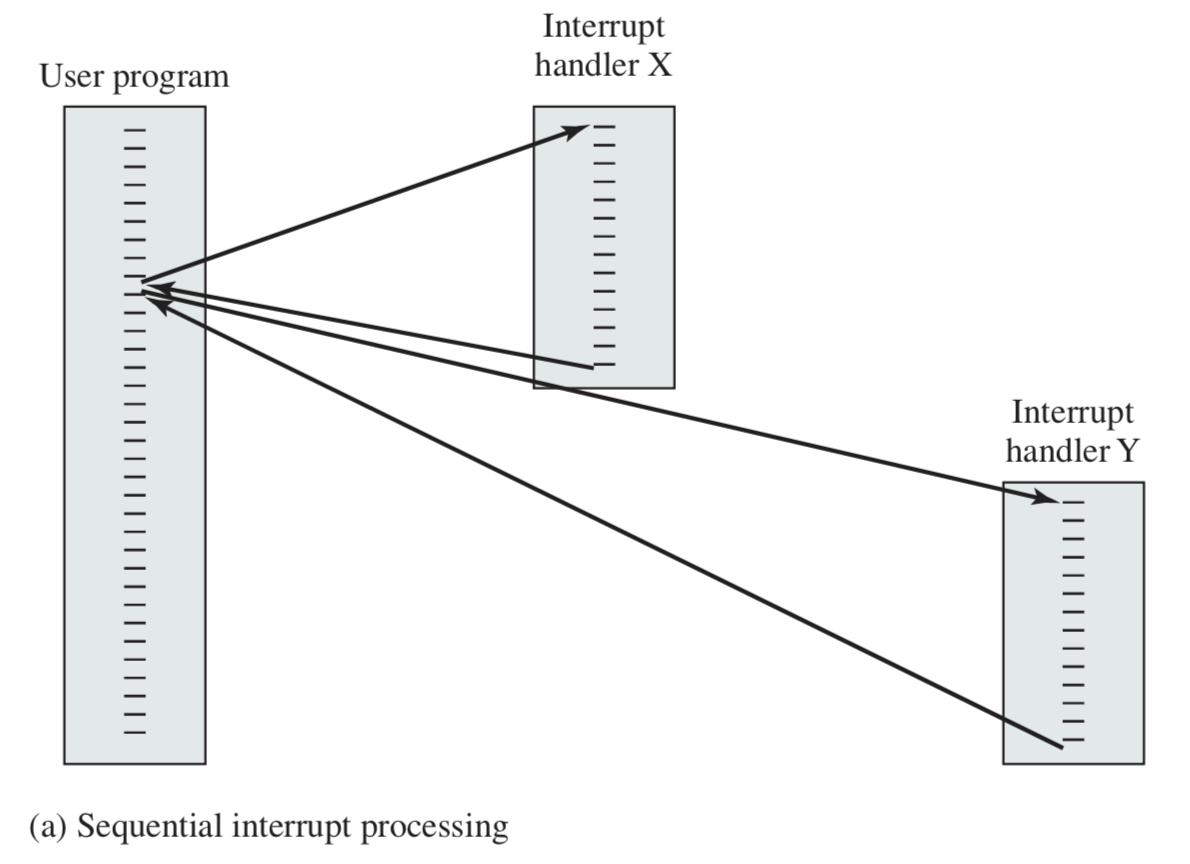
\includegraphics[width=0.8\textwidth]{images/interrupts-seq.png}
	\end{center}

	They may be sequential...

\end{frame}

\begin{frame}
	\frametitle{Interrupts}

	\begin{center}
		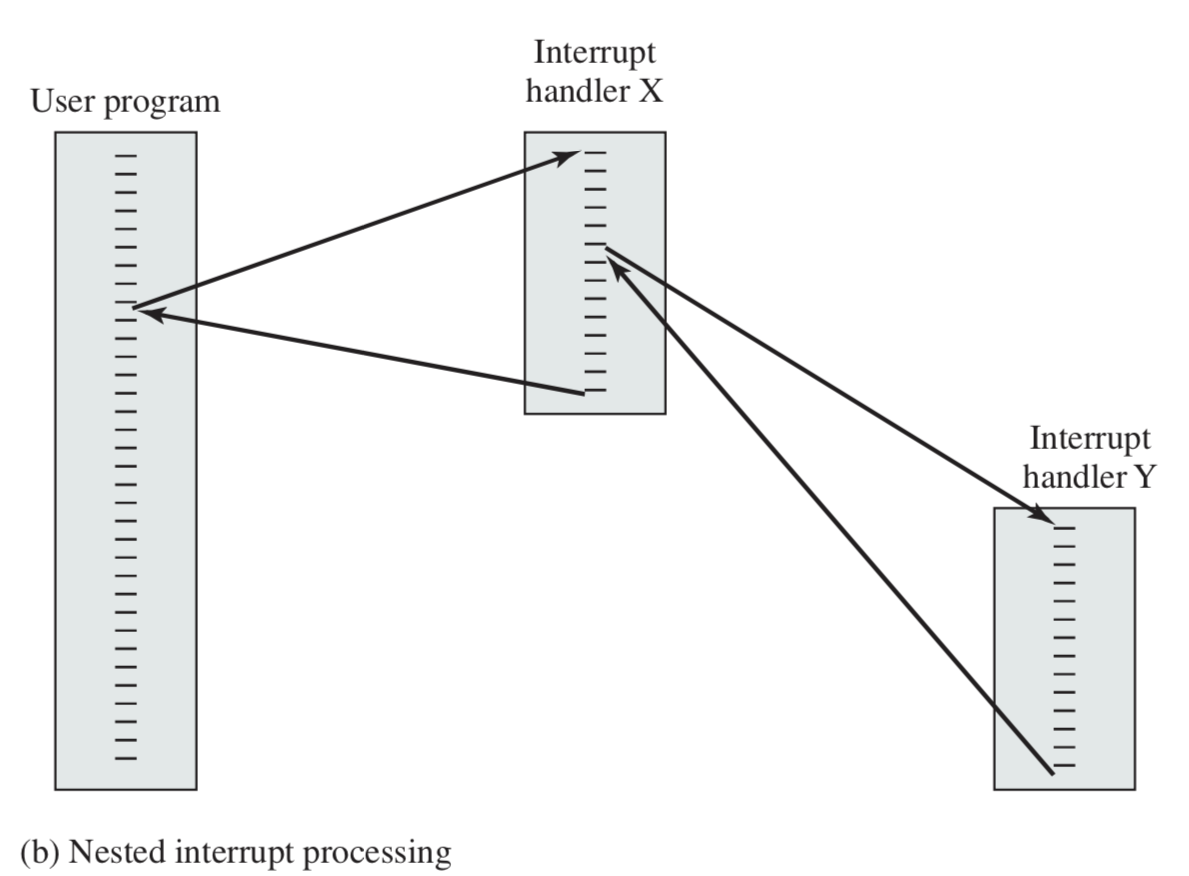
\includegraphics[width=0.8\textwidth]{images/interrupts-nest.png}
	\end{center}

	Or nested. Or a combination.

\end{frame}

\begin{frame}
	\frametitle{Storing and Restoring State}

	The OS must store the program state when an interrupt occurs.

	The state must be stored.

	State: values of registers.

	Push them onto the stack.

	Interrupt finished: restore the state (pop off the stack).

	Then execution continues.

\end{frame}

\begin{frame}
	\frametitle{Multiprogramming}
	That is saving and restoring the same program.

	Why not restore a different program?

	Scheduling decision!


\end{frame}

\begin{frame}
	\frametitle{Invoking System Calls}

	Some services run automatically, without user intervention.

	In other cases, we want specifically to invoke them. How?

\end{frame}


\begin{frame}
	\frametitle{Admiral Ackbar Says:}

	\begin{center}
		
\includegraphics[width=0.8\textwidth]{images/itsatrap.jpg}
	\end{center}

\end{frame}


\begin{frame}
	\frametitle{Trap}

	Operating systems run on the basis of interrupts.

	A \alert{trap} is a software-generated interrupt.

	Generated by an error (invalid instruction) or user program request.

\end{frame}

\begin{frame}
	\frametitle{Trap}

	If it is an error, the OS will decide what to do.\\
	\quad Usual strategy: give the error to the program.

	The program can decide what to do if it can handle it.\\
	\quad Often times, the program doesn't handle it and just dies.

\end{frame}

\begin{frame}
	\frametitle{User Mode and Kernel Mode}

	Consider: User mode vs. supervisor (kernel) mode instructions.

	Supervisor mode allows all instructions and operations.

	Even something seemingly simple like reading from disk or writing to console output requires privileged instructions.

	These are common operations, but they involve the OS every time.


\end{frame}

\begin{frame}
	\frametitle{User Mode and Kernel Mode}

	Modern processors track what mode they are in with the mode bit.

	At boot up, the computer starts up in kernel mode as the operating system is started and loaded.

	User programs are always started in user mode.

	When a trap or interrupt occurs, and the operating system takes over, the mode bit is set to kernel mode.

	When it is finished the system goes back to user mode before the user program resumes.


\end{frame}


\begin{frame}
	\frametitle{Example: Text Editor Printing}

	Suppose a text editor wants to output data to a printer.

	\begin{center}
		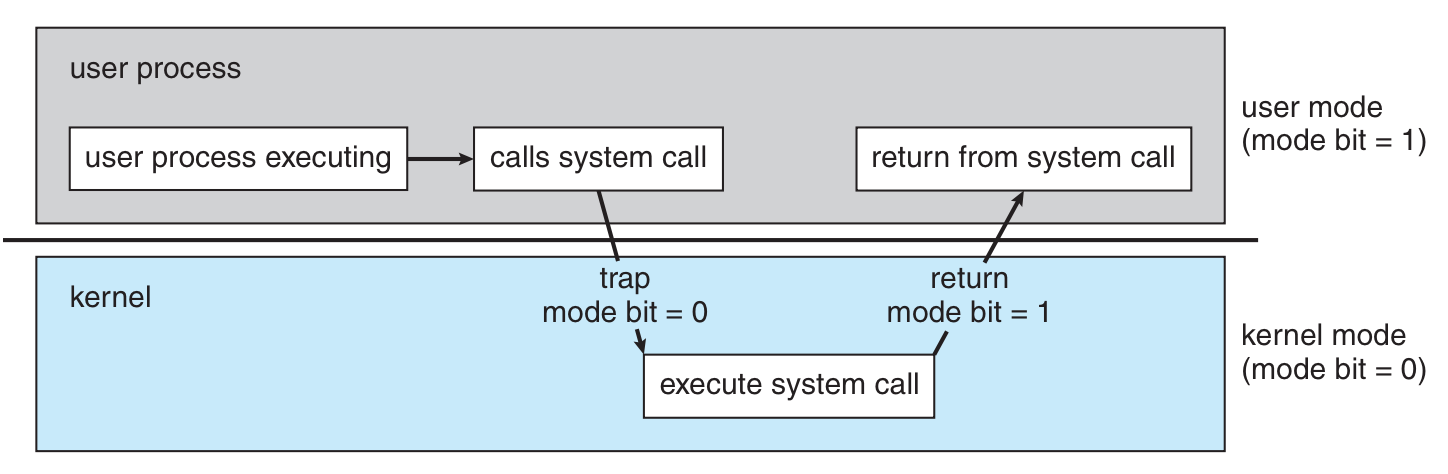
\includegraphics[width=0.9\textwidth]{images/trap.png}
	\end{center}

\end{frame}

\begin{frame}
	\frametitle{User Mode and Kernel Mode: Motivation}

	Why do we have user and supervisor modes, anyway?

	Uncle Ben to Spiderman:
	\begin{center}
		
\includegraphics[width=0.5\textwidth]{images/spiderman.jpg}
	\end{center}

\end{frame}

\begin{frame}
	\frametitle{User Mode and Kernel Mode: Motivation}


	Actually, though: ``with great power comes great responsibility''.


	Same as why we have user accounts and administrator accounts.

	To protect the system \& its integrity against errant and malicious users.


\end{frame}

\begin{frame}
	\frametitle{User Mode and Kernel Mode: Motivation}

	Multiple programs might be trying to use the same I/O device at once.

	Program~1 tries to read from disk. This takes some time.

	If Program~2 wants to read from the same disk, the operating system forces Program~2 to wait its turn.

	Without the OS, it would be up to the author(s) of Program~2 to check and wait patiently for it to become available.

	Works if everyone plays nicely.

	Without enforcement of the rules, a program will do something nasty.

\end{frame}

\begin{frame}
	\frametitle{User Mode and Kernel Mode: Motivation}

	There is a definite performance trade-off.

	Switching from user to kernel mode takes time.

	The performance hit is worth it for the security.

\end{frame}

\begin{frame}[fragile]
	\frametitle{UNIX Example: Reading from Disk}
	
Here's the function we use for reading data from a file:
	
		\begin{lstlisting}[language=C]
ssize_t read( int file_descriptor, void *buffer, size_t count );
		\end{lstlisting}


	\texttt{read} takes three parameters:
	\begin{enumerate}
		\item the file (a file descriptor, from a previous call
		      to \texttt{open});
		\item where to read the data to; and
		\item how many bytes to read.
	\end{enumerate}
	
	Example:

		\begin{lstlisting}[language=C]
int bytesRead = read( file, buffer, numBytes );
		\end{lstlisting}


	Note that \texttt{read} returns the number of bytes successfully read.

\end{frame}


\begin{frame}
\frametitle{They Elected Me To Lead, Not To Read}

This is a system call, and system calls have documentation.\\
\quad Finding and reading this information is a key skill for systems programming.

Google (or other search engine of your choice) is your friend.

Good sources: man7.org, linux.die.net, or the website of the code library!

\end{frame}


\begin{frame}
	\frametitle{Example: Reading from Disk}

	In preparation for a call to \texttt{read} the parameters are pushed on the stack.\\
	\quad This is the normal way in which a procedure is called in C(++).

	\texttt{read} is called; the normal instruction to enter another function.

	The \texttt{read} function will put its identifier in a predefined location.

	Then it executes the \texttt{trap} instruction, activating the OS.

\end{frame}

\begin{frame}
	\frametitle{Example: Reading from Disk}


	The OS takes over and control switches to kernel mode.

	Control transfers to a predefined memory location within the kernel.

	The trap handler examines the request: it checks the identifier.

	Now it knows what system call request handler should execute: read.

	That routine executes.

	When it is finished, control will be returned to the \texttt{read} function.\\
	\quad Exit the kernel and return to user mode.

	\texttt{read} finishes and returns, and control goes back to the user program.


\end{frame}


\begin{frame}[fragile]
	\frametitle{System Call Complex Example}

	\begin{lstlisting}[language=C]
#include <stdio.h>
#include <stdlib.h>
#include <unistd.h>
#include <string.h>
#include <fcntl.h>

void readfile( int fd );

int main( int argc, char** argv ) {
    if ( argc != 2 ) {
        printf("Usage: %s <filename>\n", argv[0]);
        return -1;
    }
    int fd = open( argv[1], O_RDONLY );
    if ( fd == -1 ) {
        printf("Unable to open file! %s is invalid name?\n", argv[1] );
        return -1;
    }
    readfile( fd );
    close( fd );
    return 0;
}
\end{lstlisting}
\end{frame}

\begin{frame}[fragile]
	\frametitle{System Call Complex Example}

	\begin{lstlisting}[language=C]
void readfile( int fd ) {
    int buf_size = 256;
    char* buffer = malloc( buf_size );
    while ( 1 ) {
        memset( buffer, 0, buf_size );
        int bytes_read = read( fd, buffer, buf_size - 1 );  
        if ( bytes_read == 0 ) {
            break; 
        }     
        printf("%s", buffer);
    }
    printf("\nEnd of File.\n");
    free( buffer );
}
\end{lstlisting}


\end{frame}


\begin{frame}
	\frametitle{System Call Summary}

	The steps, arranged chronologically, when invoking a system call are:
	\begin{enumerate}
		\item The user program pushes arguments onto the stack.
		\item The user program invokes the system call.
		\item The system call puts its identifier in the designated location.
		\item The system call issues the \texttt{trap} instruction.
		\item The OS responds to the interrupt and examines the identifier in the designated location.
		\item The OS runs the system call handler that matches the identifier.
		\item When the handler is finished, control exits the kernel and goes back to the system call (in user mode).
		\item The system call returns control to the user program.

	\end{enumerate}


\end{frame}

\begin{frame}
\frametitle{What about in the Cortex M4?}

The Cortex uses the function \texttt{SVC}.\\
\quad Other systems like x86 have different ones, and sometimes multiple.

User programs don't usually call \texttt{SVC} directly, but instead call an API and that wraps the system call.

Example: In Linux we call \texttt{malloc()} from \texttt{stdlib.h}, but it may call the \texttt{brk} system call (and this contains the trap).

\end{frame}

\begin{frame}
\frametitle{Cortex Syscall Framework}

The \texttt{SVC} instruction takes one integer in the range \texttt{0 - 255}.

This argument is the ``identifier'' in the ``predefined location'' from earlier.

We get to choose the meanings of the numbers:\\
\begin{itemize}
	\item 0 = print something
	\item 1 = switch threads
	\item 2 = wait for input
	\item ...
\end{itemize}

\end{frame}

\begin{frame}
\frametitle{Now What}

\begin{center}
  
\includegraphics[width=0.5\textwidth]{images/sleeper.png}
\end{center}

Next: Run the \texttt{SVC\_Handler} (Assembly Code):\\
\quad Extract the integer parameter, invoke the C function

Then: Run \texttt{SVC\_Handler\_Main} (C Code):\\
\quad Call the individual system call corresponding to the parameter.

\end{frame}

\begin{frame}[fragile]
\frametitle{Activating the System Call}

Inside our C code, use embedded assembly. To invoke system call \texttt{1}:

\begin{lstlisting}[language=C]
__ASM("SVC #1");
\end{lstlisting}

The \# is required! 

Remember: we choose the number and what it does on the other side.
\end{frame}

\begin{frame}[fragile]
\frametitle{Getting to C}

Don't write this down, but here's the \texttt{SVC\_Handler} ASM:

\begin{lstlisting}
AREA handle_pend,CODE,READONLY
GLOBAL SVC_Handler
PRESERVE8

SVC_Handler
    ;We will be calling this function to handle the various system calls
    EXTERN SVC_Handler_Main
    
    ;Check the magic value stored in LR to determine whether we are in thread mode
    TST LR,#4 ;check the magic value
    ITE EQ ; If-Then-Else
    MRSEQ r0, MSP ; If LR was called using MSP store MSP's value in r0
    MRSNE r0, PSP ; Else store PSP's value
    
    BL SVC_Handler_Main ;Jump to the C function which handles the system calls
    
    END
\end{lstlisting}

\end{frame}


\begin{frame}[fragile]
\frametitle{Start of the C Function}
Warning: we're about to do some weird things to the stack.

\begin{lstlisting}[language=C]
void SVC_Handler_Main( uint32_t *svc_args) {
    /* ARM sets up the stack frame so that the syscall number is two
       characters behind the input argument */
    char call = ((char*)svc_args[6])[-2];
    
    /* Now decide what to do with call (if or switch statement)
       eg if ( call == 0 ) { ... } */

}
\end{lstlisting}

\end{frame}

\begin{frame}
\frametitle{Now Wait a Minute}

This framework is very basic, and is missing a few things.

There's no way to pass arguments from user programs to system calls...\\
\quad And no way to return arguments either.

The introduction to the UNIX system call suggested how to do this (stack).

For now, we'll use shared memory areas.

\end{frame}

\begin{frame}
\frametitle{Shared Memory?}

\begin{center}
  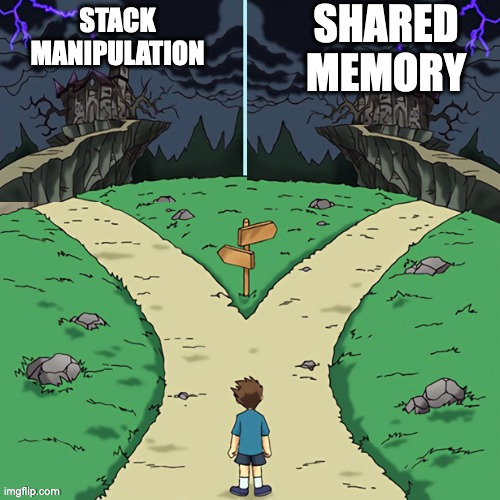
\includegraphics[width=0.4\textwidth]{images/twocastles.jpg}
\end{center}

Shared memory areas are a headache too.

Shared memory areas must be limited in size and protected (1 per thread).

\end{frame}

\begin{frame}
\frametitle{Does it Work?}

We need to get to Kernel mode and \texttt{SVC} is an interrupt.\\
\quad Interrupts run in kernel mode!

Our rudimentary implementation is very insecure.

For fun: try to hack it: can you inject code to a syscall or hijack shared memory?

\end{frame}


\end{document}

